\documentclass[a4paper,11pt]{book}
\usepackage[centertags]{amsmath}
\usepackage{amscd}
\usepackage{amsthm}
\usepackage{amssymb}
\usepackage{enumerate}
\usepackage[dvips]{graphics}
\usepackage{graphicx, subcaption} % takes care of graphic including machinery
\usepackage{algorithm}
\usepackage{algpseudocode} 
\usepackage{multicol}
\usepackage{hyperref}
\usepackage[english]{babel}
\usepackage{color}
\usepackage{tikz}
\usepackage{tabls} %per tenir m{\'e}s control sobre l'espai en les taules nom{\'e}s cal aquest paquet
\usepackage{indentfirst} %per comen\c{c}ar primer parragraf de seccio o capitol amb indent
\usepackage{imakeidx}
\usepackage{caption}
\captionsetup{width=.9\textwidth}

\makeindex
\usepackage[T1]{fontenc}
\linespread{1.1} % Palatino needs more leading (space between lines)

\usepackage[latin1]{inputenc}
\usepackage[twoside,bindingoffset=1cm]{geometry}


%%%%%%%%%%%%%%%%%%%%%%%%%%%%%%%%%%%%%%%%%%%%%%%%%%%%%%%%%%%%%%%%%%%%%%%%%
% theorem environments
%%%%%%%%%%%%%%%%%%%%%%%%%%%%%%%%%%%%%%%%%%%%%%%%%%%%%%%%%%%%%%%%%%%%%%%%%
\newtheorem{defn0}{Definition}[chapter]
\newtheorem{prop0}[defn0]{Proposition}
\newtheorem{thm0}[defn0]{Theorem}
\newtheorem{lemma0}[defn0]{Lemma}
\newtheorem{corollary0}[defn0]{Corollary}
\newtheorem{example0}[defn0]{Example}
\newtheorem{remark0}[defn0]{Remark}
\newtheorem{conjecture0}[defn0]{Conjecture}
\newtheorem{prob0}[defn0]{Problem}

\newenvironment{definition}{ \begin{defn0}}{\end{defn0}}
\newenvironment{proposition}{\bigskip \begin{prop0}}{\end{prop0}}
\newenvironment{theorem}{\bigskip \begin{thm0}}{\end{thm0}}
\newenvironment{lemma}{\bigskip \begin{lemma0}}{\end{lemma0}}
\newenvironment{corollary}{\bigskip \begin{corollary0}}{\end{corollary0}}
\newenvironment{example}{ \begin{example0}\rm}{\end{example0}}
\newenvironment{remark}{ \begin{remark0}\rm}{\end{remark0}}
\newenvironment{conjecture}{\begin{conjecture0}}{\end{conjecture0}}
\newenvironment{problem}{\begin{prob0}}{\end{prob0}}

\newcommand{\defref}[1]{Definition~\ref{#1}}
\newcommand{\propref}[1]{Proposition~\ref{#1}}
\newcommand{\thmref}[1]{Theorem~\ref{#1}}
\newcommand{\lemref}[1]{Lemma~\ref{#1}}
\newcommand{\corref}[1]{Corollary~\ref{#1}}
\newcommand{\exref}[1]{Example~\ref{#1}}
\newcommand{\secref}[1]{Section~\ref{#1}}
\newcommand{\remref}[1]{Remark~\ref{#1}}
\newcommand{\conjref}[1]{Conjecture~\ref{#1}}
\newcommand{\probref}[1]{Problem~\ref{#1}}


%%%%%%%%%%%%%%%%%%%%%%%%%%%%%%%%%%%%%%%%%%%%%%%%%%%%%%%%%%%%%%%%%%%%%%%%%%%
%%%% local definitions for this paper
%%%%%%%%%%%%%%%%%%%%%%%%%%%%%%%%%%%%%%%%%%%%%%%%%%%%%%%%%%%%%%%%%%%%%%%%%%%

\newlength{\cellheight}
\setlength{\cellheight}{\dimexpr 3\baselineskip / 4\relax}

% monomio
\newcommand{\mono}{\texorpdfstring{\,\vcenter{\hbox{
\includegraphics[scale=0.15]{./pictures/monomio/monomio.pdf}}}\,}.}

% dominoes
\newcommand{\VD}{\texorpdfstring{\,\vcenter{\hbox{
\includegraphics[scale=0.15]{./pictures/dominoes/v-domino.pdf}}}\,}i}
\newcommand{\HD}{\texorpdfstring{\,\vcenter{\hbox{
\includegraphics[scale=0.15]{./pictures/dominoes/h-domino.pdf}}}\,}i}

% triminoes
\newcommand{\Itri}{\texorpdfstring{\,\vcenter{\hbox{
\includegraphics[scale=0.15]{./pictures/trimonios/I3.pdf}}}\,}I}
\newcommand{\Ltri}{\texorpdfstring{\,\vcenter{\hbox{
\includegraphics[scale=0.15]{./pictures/trimonios/L3.pdf}}}\,}L}


% tetrominoes
\newcommand{\OO}{\texorpdfstring{\,\vcenter{\hbox{
\includegraphics[scale=0.15]{pictures/tetrominos/O.pdf}}}\,}O}
\newcommand{\TT}{\texorpdfstring{\,\vcenter{\hbox{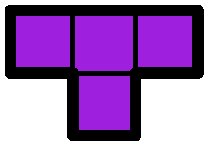
\includegraphics[scale=0.15]{pictures/tetrominos/T.pdf}}}\,}T}
\newcommand{\LL}{\texorpdfstring{\,\vcenter{\hbox{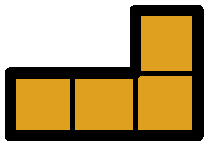
\includegraphics[scale=0.15]{pictures/tetrominos/L_90.pdf}}}\,}L}
\newcommand{\LLvert}{\texorpdfstring{\,\vcenter{\hbox{
\includegraphics[scale=0.15]{pictures/tetrominos/L.pdf}}}\,}L}
\newcommand{\JJ}{\texorpdfstring{\,\vcenter{\hbox{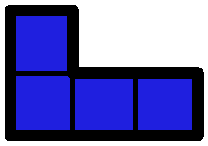
\includegraphics[scale=0.15]{pictures/tetrominos/J_90.pdf}}}\,}J}
\renewcommand{\SS}{\texorpdfstring{\,\vcenter{\hbox{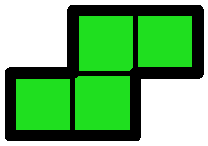
\includegraphics[scale=0.15]{pictures/tetrominos/S.pdf}}}\,}S}
\newcommand{\ZZ}{\texorpdfstring{\,\vcenter{\hbox{
\includegraphics[scale=0.15]{pictures/tetrominos/Z.pdf}}}\,}Z}
\newcommand{\II}{\texorpdfstring{\,\vcenter{\hbox{
\includegraphics[scale=0.15]{pictures/tetrominos/I_90.pdf}}}\,}I}

\newcommand{\ALL}{\II, \allowbreak \OO, \allowbreak \TT, \allowbreak \SS, \allowbreak \ZZ, \allowbreak \JJ, \allowbreak \LL}


\NewDocumentCommand{\cell}{O{i} O{j}}{
 \langle #1, #2 \rangle
}
\NewDocumentCommand{\piece}{O{t} O{\theta} O{i} O{j} O{f}}{
 (#1, \allowbreak #2, \allowbreak \langle #3, \allowbreak #4 \rangle,  \allowbreak #5 )
}

\newcommand{\texttheo}[1]{\textnormal{\textsf{#1}}}
\newcommand{\tetris}[1]{\textsc{Tetris}[#1]\xspace}
\newcommand{\npc}{\textnormal{\textsf{NP-complete}}}
\newcommand{\np}{\textnormal{\textsf{NP}}}
\newcommand{\pp}{\textnormal{\textsf{P}}}
\newcommand{\nph}{\textnormal{\textsf{NP-hard}}}
\newcommand{\survival}{$\texttheo{survival}$}
\newcommand{\clearing}{$\texttheo{clearing}$}


%%%%%%%%%%%%%%%%%%%%%% aixo pels headings %%%%%%%%%%%%%%%%%%%%%%%%
\setlength{\headheight}{14.5pt}
\usepackage{fancyhdr}
\pagestyle{fancy}
\renewcommand{\chaptermark}[1]{\markboth{#1}{}}
\renewcommand{\sectionmark}[1]{\markright{\thesection\ #1}}
\fancyhf{} \fancyhead[LE,RO]{\bfseries\thepage}
\fancyhead[LO]{\bfseries\rightmark} 
\fancyhead[RE]{\bfseries\leftmark}

\def\paginaenblanc{\newpage%
\thispagestyle{empty}%
\vspace*{2cm}%
\newpage%
\thispagestyle{empty}%
}


%%%%%%%%%%%%%%%%%%%%%%%%%%%%%%%%%%%%%%%%%%%%%%%%%%%%%%%%%%%%%%%%%%%%%%%%%
% aux commands
%%%%%%%%%%%%%%%%%%%%%%%%%%%%%%%%%%%%%%%%%%%%%%%%%%%%%%%%%%%%%%%%%%%%%%%%%
%==========================================================================
% macros to support private authors' notes
%==========================================================================
\newif\ifprivate
\privatetrue
\def\xbar{\vskip0.09in\hrule\vskip0.06in}
\def\private#1{\ifprivate \xbar {\em #1} \xbar
\else \fi}
\def\huh{\ifprivate ??? \marginpar{\Huge ???}
\else \fi}
\def\???{\ifprivate {\bf {???}} \marginpar{\begin{center}{\Huge {\bf ?}}\end{center}}
\else \fi}
%\def\???{\ifprivate {\bf {???}} \marginpar{{\Huge {\bf ?}}}
%\else \fi}
\marginparsep1mm
\def\nota#1{\ifprivate  $\clubsuit$ \marginpar{\parbox[t]{2.4cm}{\begin{center}\tiny #1\end{center}}}
\else \fi}
\def\comment#1{\ifprivate \marginpar{\parbox[t]{2.4cm}{\begin{center}\tiny #1\end{center}}}
\else \fi}
%\def\nota#1{\ifprivate  $\clubsuit$ \marginpar{\parbox[t]{1.8cm}{\tiny #1}}
%\else \fi}
\def\privateeject{\ifprivate\eject\fi}
%\def\???{{\bf {???}} \marginpar{{\Huge {\bf ?}}} }
%%%%%%%%%%%%%%%%%%%%%%%%%%%%%%%%%%%%%%%%%%%%%%%%%%%%%%%%%%%%%%%%%%%%%%%%%%

%%%%%%%%%%%%%% definicions cap{\'\i}tol ""%%%%%%%%
%%%%%%%%%%%%%%%%%%%%%%%%%%%%%%%%%%
\def\av{\underline{a}}

\def\Zr{\mathbb Z^r} \def\Nr{\mathbb N^r}
\def\xv{\underline{x}}
\def\yv{\underline{y}}
\def\zv{\underline{z}}

\newcommand{\Proj}{\operatorname{Proj}}
\newcommand{\Spec}{\operatorname{Spec}}


\def\HiRIM#1{H^i_{\mathcal M}(#1)}

\newcommand{\im}{\operatorname{Im}}
\renewcommand{\ker}{\operatorname{Ker}}
\newcommand{\grade}{\operatorname{grade}}
\newcommand{\Ext}{\operatorname{Ext}}
\newcommand{\Hom}{\operatorname{Hom}}
\newcommand{\m}{\mathfrak m}
\newcommand{\n}{\mathfrak n}
\newcommand{\M}{\mathfrak m}
%\newcommand{\cL}{{\mathcal L}}
\newcommand{\cP}{{\mathcal P}}
\newcommand{\cE}{{\mathcal E}}
\newcommand{\cS}{{\mathcal S}}
\newcommand {\PP}{\mathbb{P}}

\def\p{\mathfrak{p}}
\def\q{\mathfrak{q}}
\DeclareMathOperator{\de}{deg}

\DeclareMathOperator{\Hl}{H}
 \DeclareMathOperator{\h}{h}


%%%%%%%%%%%%%%%%%%%%%%%%%%%%%%%%%%%%%%%%%%%%%%%%%%%%%%%%%%%%%%%%%%%%%%%%
\begin{document}

\makeatletter
\def\old@comma{,}
\catcode`\,=13
\def,{%
  \ifmmode%
    \old@comma\discretionary{}{}{}%
  \else%
    \old@comma%
  \fi%
}
\makeatother


\begin{titlepage}
\begin{center}
\begin{figure}[htb]
\begin{center}
  
\includegraphics[width=6cm]{./pictures/matematiquesinformatica-pos-rgb.png}
\end{center}
\end{figure}

\vspace*{1cm}
\textbf{\LARGE GRAU DE MATEM\`{A}TIQUES } \\
\vspace*{.5cm}
\textbf{\LARGE Treball final de grau} \\



\vspace*{1.5cm}
\rule{16cm}{0.1mm}\\
\begin{Huge}
\textbf{Complexitat del Tetris} \\
\end{Huge}
\rule{16cm}{0.1mm}\\

\vspace{1cm}

\begin{flushright}
  \textbf{\LARGE Autor: Pol Ros Dom\`{e}nech}

\vspace*{2cm}

\renewcommand{\arraystretch}{1.5}
\begin{tabular}{ll}
\textbf{\Large Director:} & \textbf{\Large Dr. Kolja Knauer} \\
\textbf{\Large Co-Directora:} & \textbf{\Large Dr. Carme \`Alvarez Faura} \\
\textbf{\Large Realitzat a:} & \textbf{\Large  Departament Matem\`{a}tica Aplicada } \\
\textbf{\Large Barcelona,} & \textbf{\Large \today }
\end{tabular}

\end{flushright}

\end{center}

\end{titlepage}

\tableofcontents
%%%%%%%%%%%%%%%%%%%%% aix{\`o} pels headings %%%%%%%%%%%%%%%%%%%%%%%%

\newpage



\section*{Abstract}

The computational complexity of Tetris has been extensively studied across various problem formulations and game variations, most of which are classified as NP-hard. This paper explores the fundamental factors contributing to this complexity. We begin by generalizing the Tetris problem, parametrizing its key components to create a unified framework for all variations. Next we examine existing research and identify critical findings about each variant. After the analysis, we focus on a specific variation of Tetris with dominoes, addressing the open problem of survival by demonstrating that it is solvable in polynomial time. In doing so, we provide new insights into the mechanisms driving the complexity of Tetris and its variants. Additionally, we present progress on several other open problems related to Tetris with dominoes, contributing further to the understanding of its computational challenges.

{\let\thefootnote\relax\footnote{2020 mathematics subject classification. 68W99, 68Q25, 68-02}}


\mainmatter

Tetris, created in 1984 by Alexey Pajitnov, .... 


A lot of work has been done around Tetris. In fields such as computer science, it has been studied for its algorithmic complexity, AI applications, and programming education. Studies on human interaction with Tetris explore cognitive processes, social behaviors, and performance factors. Additionally, Tetris has influenced robotics, narrative storytelling, and educational tools, while its theoretical challenges, such as NP-completeness, continue to intrigue researchers \cite{TWRP}.


the question \emph{"what makes Tetris hard?"} or \emph{"where is the complexity in tetris?"}.


\section{Game Definitions}

In \cite{TIH} we can find a formalization of the Tetris game and a decisional/functional problem associated to it. Since the video game is played in finite board and a player can't win, the definition of the game introduces some variations to build a complexity problem.

In \cite{TT,TWFP,TCB,CTV,AVG} game variations are introduced without any formalization of the new emerging problems. We are going to provide a generalized Tetris game definition, following \cite{TIH}, which aims to include all possible game variations and the combination of these. Right after defining each part of the game, an example will be given of what be in the video game and what it is in the definition of \cite{TIH}. We will refer to \emph{video game} and \emph{base tetris} respectively.

A \emph{Tetris game} will refer to the hole game with its rules, configurations, pieces, ... and a \emph{tetris match} will refer to a concrete Tetris game instance (the sequence of moves that a player would play). 

\begin{definition} \index{board}
  A \emph{board} \emph{B} is an $n$ by $m$ grid. Each cell $\cell$, $i = 1\dots n$, $j = 1\dots m$ is \emph{filled} or \emph{unfilled}.
\end{definition}

The board will be indexed from bottom to top and from left to right. The cell $\cell[1][1]$ is in the bottom left of the board and $\cell[n][m]$ is the top right-most cell.

In some results, the authors impose that the initial configuration must be constructible with the pieces and the rules of the game. This is that the initial configuration can be reached, with the game rules, from an empty board and an appropriate pieces sequences. Others, the only condition that is imposed on the initial configuration is that it can't have filled rows. We will not impose the board to be constructible, (parlem despres).

\begin{example} 
  \begin{itemize}
    \item \textbf{Video game:} the board size is typcaly a unfilled 10x20 board.
    \item \textbf{Base Tetris: } the board size has arbitrary dimensions.
  \end{itemize}
\end{example}


Tetris classical pieces are made up by attaching 4 squares. In the variations we can find pieces types, in a game there are usually pieces with the same number of cubes. A general Tetris piece made up with $k$ cells is:

\begin{definition} \index{$k$-omino} \index{polymonio}
  A \emph{$k$-omino} is a piece made up of $k$ unit squares joined edge to edge. A \emph{polyomino} is a $k$-omino for some $k$.
\end{definition}

For $k= 1,2,3,4,5$ the $k$-omio pieces are called respectively: \emph{monomino}, \emph{domino}, \emph{tromino}, \emph{tetromino} and \emph{pentomino}.

\begin{definition} \index{piece!types}
  The \emph{piece types} $T$ is a set of polyominos. If $T$ contains all the $k$-omions we will write $T_k$.
\end{definition}

\begin{example} The \textbf{video game} and the \textbf{base Tetris} have the same  pieces types $T_4 = \{ \ALL \}$, all the tetrominoes.
\end{example}

Given the pieces and the board, we can now define how a piece interacts with a board. 

\begin{definition} \index{piece!state} \index{piece}
 A \emph{piece state} in a board $B$ is a tuple $ P = \piece$ where:
  \begin{itemize}
    \item $t \in T$, a polyomino.
    \item $\theta$ the \emph{orientation}, the number of degrees clockwise from the original piece. $ \theta \in \lbrace 0^\circ, 90^\circ, 180^\circ, 270^\circ \rbrace $.
    \item $\cell$ is the \emph{position} of the piece in of $B$
    \item  $f$ indicates if the piece is \emph{fixed} or \emph{unfixed} in B.
  \end{itemize}

  We will refer to a piece sate as \emph{piece}.
   
\end{definition}


\begin{definition}
  Given a piece type $t$ and a board $B$, the piece $P_0 = \piece[t][0^\circ][n][\lfloor m / 2 \rfloor][\text{unfixed}]$ is the \emph{initial state} of the piece type of $t$ in the board $B$.
\end{definition}

The idea is to have only one active piece in a Tetris match. Only the piece that is moving has a state because when a piece reaches the \emph{fixed} state the piece is automatically merged with the board, and then the next piece starts in its initial state. In order to define how a piece moves thought the board, we need to define some \emph{moves} for changing the piece state.

\begin{definition}
  A \emph{move} is a computable function $m(B, P) = P'$ that given a board $B$ and a piece $P$ outputs a new piece $P'$. The following moves can be applied to an unfixed piece $P = \piece[t][\theta][i][j][\text{unfixed}]$. 
  \begin{itemize}
    \item $r_+$ a \emph{clockwise rotation:} if the rotated piece does not overlap with an occupied cell of the board, the output is 
      $$r_+ (B, \piece[t][\theta][i][j][\text{unfixed}]) = \piece[t][\theta + 90^\circ][i][j][\text{unfixed}]$$

    \item $r_-$ a \emph{counterclockwise rotation:} the same but counterclockwise rotation. 

    \item $s_l$ a \emph{slide to the left:} if all the board cells adjacent to de left of the piece are not occupied, the output is:
      $$s_l (B, \piece[t][\theta][i][j][\text{unfixed}]) = \piece[t][\theta][i][j-1][\text{unfixed}]$$
    \item $s_r$ a \emph{slide to the right:} analogous to the slide to the left.

    \item $d$ a \emph{drop by one row:} if all the board cells bellow the piece are not occupied the output is:
      $$d (B, \piece[t][\theta][i][j][\text{unfixed}]) = \piece[t][\theta][i-1][j][\text{unfixed}]$$

    \item $f$ a \emph{fix:} if any of the board cells bellow the piece is occupied, the output is:
      $$f (B, \piece[t][\theta][i][j][\text{unfixed}]) = \piece[t][\theta][i][j][\text{fixed}]$$
  \end{itemize}
  If the pre-conditions of a move are satisfied, the move is said to be \emph{legal}. If any of the conditions are not satisfied the move is \emph{illegal}.
\end{definition}

All the conditions can be computed in $\mathcal{O}(1)$, because only a constant numbers of cells are need to be visited every time. Let's now define the \emph{trajectory} of a piece type in a Tetris game. Intuitively the trajectory starts when the piece is given to the player, consists on a sequence of legal moves and ends when he fixes the piece in the board. 


\begin{definition}
 Let $B$ be a board and $t$ a piece type. Let $P_0$ be the initial state of the piece type $t$. Then a sequence of $k$ moves $\sigma = (m_1, ..., m_k)$ to the piece state after $i$ moves is a \emph{trajectory} if:

 \begin{itemize}
  \item the move $m_i$ over $P_i$ is a legal move for all $i = 1 \dots k$
  \item and $m_k = f$ is a \emph{fix} move.
 \end{itemize}
 
 Where $P_{i+1} = m_i(P_i)$ is the piece stat in $B$ after $i$ moves.
\end{definition}

The number of moves of a trajectory could be limited by $\mathcal{O}(n \cdot m)$?

With a board and a trajectory we need to define how we merge both. The resulting board will be the merged board. 

\begin{definition}
  Given a board $B$ and trajectory $\sigma = (m_1, ..., m_k)$ of a given piece type $t$ the \emph{merged game board} $B'$ is defined as follows:
  \begin{enumerate}
    \item $B'$ is initially $B$.
    \item The cells of $B$ corresponding to the last piece state of the trajectory are filled in $B'$.
    \item For every filled row $r$ of $B'$:
      \begin{enumerate}
        \item Replace each row $r' > r$ by $r'+1$.
        \item Clear (set all cells to unfilled) of row $m$.
      \end{enumerate}
  \end{enumerate}
\end{definition}

We have now all the components of a Tetris match.

\begin{definition}
  Given a board $B$ and a sequence of $k$ pieces types $P = (t_1,\dots,t_k)$ a \emph{Tetris match} $\Sigma$ is a sequence
  $$ B = B_0, \sigma_1, B_1, \sigma_2, B_2, \dots  \sigma_q, B_q, \; \; q \leq k$$ 
  where:
  \begin{itemize}
    \item $\sigma_i$ is a trajectory of the piece type $t_i$ in the board $B_{i-1}$.
    \item $B_{i+1}$ is the merged board from $B_i$ and $\sigma_i$.
    \item $q < k$ iff doesn't exist any trajectory $\sigma_{q+1}$ from de board $B_q$ with the piece type $t_{q+1}$. In this case we say the game is a \emph{loss}.
  \end{itemize}
\end{definition}

\section{Problem}

All the problems share the same formulation of the problem. The \textsc{Tetirs} problem is:

\begin{itemize}
  \item \textbf{Input} (\textit{a Tetris game}) : $\mathcal{G} = (B,(t_1,\dots,t_k))$ an initial board and a sequence of $k$ pieces types.
  
  \item \textbf{Output} : Does exist a match $\Sigma$ such that $\Phi ( \mathcal{G}, \Sigma )$ holds? 
\end{itemize}

Where $\Phi(\mathcal{G},\Sigma)$ is computable objective function that only takes into account the final state of the pieces, ignoring the piece trajectory (\emph{checkable and acyclic}). 


We will divide the problem variants classification in two parts: variations on the objective function and variations on the game formulation.

\subsection{Objective functions} 

Will refer to the \textsc{Tetris} problem with the objective function $\Phi$ as $\textsc{Tetris} [ \Phi ]$. The following are objective functions:

\begin{itemize}
  \item \texttheo{k-cleared-rows}: in the game $\mathcal{G}$, does $\sigma$ clear at least $k$ rows?
  \item \texttheo{k-tetrises}: in the game $\mathcal{G}$, does $\sigma$ contain at least $k$ tetrises?
  \item \texttheo{h-height-filled}: in the game $\mathcal{G}$, does $\sigma$ never fill a cell above height $h$?
  \item \texttheo{p-placed-pices}: in the game $\mathcal{G}$, does $\sigma$ place at least $p$ pieces before losing.
\end{itemize} 

The two most popular variations are:

\begin{itemize} 
  \item \clearing: in the game $\mathcal{G}$, does $\sigma$ leave every cell of the board unfilled?
  \item \survival: is equivalent to \texttheo{n-height-filled}, where $n$ is the height of board $B$. This is finding a sequence $\Sigma$ that is not a loss.
\end{itemize}

\section{Game variations and Results}

Game variations are obtained tweaking definitions of the game. The following parameters of the game can be changed: 

\begin{itemize}
  \item \textbf{Pieces:} changing the pieces set of a Tetris game
  \item \textbf{Moves:} extending, reducing or changing the moves that can be applied to the pieces. 
  \item \textbf{Board:} fixing the board dimensions or impose restriction of the initial board.
  \item \textbf{Pieces sequences:} imposing restriction over the sequence of pieces.
\end{itemize}

The following papers provide results on Tetris and its variations.

\subsection{Tetris is hard, even to approximate}

The first results about Tetris complexity appear in \cite{TIH}. The results are the following:

\begin{theorem}
  Tetris is \nph to optimize (or approximate) with the objectives, \texttheo{k-cleared-rows}, \texttheo{k-tetrises} \texttheo{h-height-filled} and \texttheo{p-placed-pices}. It remains \nph even if:
  \begin{itemize}
    \item The player is restricted to two rotation/translation moves before each piece drops in height.
    \item Pieces are restricted to $\{\LL, \SS, \II, \OO\}$ or $\{\LL, \ZZ, \II, \OO\}$ plus at least one other piece.
    \item Losses are not triggered until after filled rows are cleared.
    \item Rotations follow any reasonable rotation model.
  \end{itemize}
\end{theorem}

A \emph{reasonable rotation model} is a generalization of the $\{r_+,r_-\}$ moves, extending the available rotations for a piece in a board. The two rotation functions are reasonable if some common sense conditions, defined in \cite{TIH}.

OPEN PROBLEMS?

\subsection{Total Tetris: Tetris with Monominoes, Dominoes, Trominoes, Pentominoes, ...}

In \cite{TT} a piece variation is introduced. $k$-\textsc{tris} changes the pieces types by changing the number of \emph{cells} ($k$) that form the piece types. The  set of pieces types in $k$-\textsc{tris} is all possible pieces of $k$ cells.

In the classical Tetris is $4$-\textsc{tris}, where 7 possible pieces can be built. For $k = 1$ one piece types is available (a cell), for $k=2$ also one piece type is only available (two adjacent cells), and so on. 

The formalization is almost the same as the one described in this document. The set of piece types varies depending on $k$, and each respective center. Varies depending on $k$. The \emph{moves} describing each piece state transformation is appropriately modified to fit the new piece types. Results are presented in Table~\ref{tab:tt} 


\subsubsection{Without rotation}

If we remove $r_+, r_-$ from the moves set we obtain Tetris without rotation, were the player cannot rotate pieces. Since the orientation in the \emph{initial position} of a piece is always $\theta = 0^\circ$, we can fix this by adding the initial orientation of each piece in the Tetris game instance.

\textbf{Input} (\textit{a Tetris game}): $\mathcal{G} = (B,(t_1,\theta_1, \dots,t_k,\theta_1))$ an initial board and a sequence of $k$ pieces types and its initial orientation.


The rest of the game is exactly the same. The results are presented in Table~\ref{tab:tt} 

\begin{table}[h!]
\centering
\label{tab:tt}
\begin{tabular}{|c || c | c || c | c ||} 
 \hline
  & \multicolumn{2}{| c ||}{\survival} & \multicolumn{2}{| c |}{\clearing} \\
 \hline
  & with rotation & no rotation & with rotation & no rotation \\
 \hline               
 $k = 1$ & \pp  & \pp  & \pp  & \pp \\ 
 \hline                             
 $k = 2$ & Open & Open & Open & \npc \\
 \hline                             
 $k = 3$ & Open & \npc & \npc & \npc\\
 \hline                             
 $k = 4$ & \npc & \npc & \npc & \npc\\
 \hline                             
 $k > 5$ & \npc & \npc & \npc & \npc\\
 \hline
\end{tabular}

\caption{\cite{TT} results with rotation}
\end{table}

OPEN PROBLEMS?

\subsection{Tetris is NP-hard even with O(1) rows or columns}

Following the variants introduced in \cite{TT}, in \cite{TCB} new variations are introduced. In  a $(\leq)k$-\textsc{tris} game, the set of pieces types is all possible pieces of $\leq k$ cells. Then we define the following problems:

\begin{itemize}
  \item $c$-\textsc{Column} $(\leq)k$-\textsc{tris}: $(\leq)k$-\textsc{tris} where the board width is fixed to $c$.
  \item $r$-\textsc{Row} $(\leq)k$-\textsc{tris}: $(\leq)k$-\textsc{tris} where the board height is fixed to $c$.
\end{itemize}

The rows and columns, respective, remain arbitrary. These two versions can be combined with the empty Tetris.

\begin{itemize}
  \item \textsc{Empty $(\leq)k$-\textsc{tris}}: $(\leq)k$-\textsc{tris} where all the board cells are initially unfilled.
\end{itemize}

Results with this variation are in Table~\ref{tab:tcb}

\begin{table}[h!]
\centering
\label{tab:tcb}
\begin{tabular}{|c | c | c | c | c |} 
 \hline
 Rows   & Columns & Empty  & Piece Sizes  & Complexity      \\
 \hline
 \hline
 $1   $ & $O(n) $ & no     & $O(n)    $ & strongly \nph   \\ \hline
 $1   $ & $O(n) $ & yes    & $O(n)    $ & linear          \\ \hline
 $1   $ & $O(n) $ & no     & $k       $ & linear          \\ \hline
 $2   $ & $O(n) $ & yes    & $O(n)    $ & strongly \nph   \\ \hline
 $3   $ & $O(n) $ & no     & $4       $ & Open            \\ \hline
 $4   $ & $O(n) $ & no     & $4       $ & strongly \nph   \\ \hline
 $O(n)$ & $1    $ & no     & $O(n)    $ & linear          \\ \hline
 $O(n)$ & $2    $ & no     & $O(n)    $ & polynomial      \\ \hline
 $O(n)$ & $3    $ & yes    & $O(n)    $ & strongly \nph   \\ \hline
 $O(n)$ & $3 - 7$ & no     & $4       $ & Open            \\ \hline
 $O(n)$ & $8+   $ & no     & $4       $ & strongly \nph   \\ \hline
 $O(n)$ & $8    $ & yes    & $\leq 65 $ & strongly \nph   \\
 \hline
\end{tabular}
\caption{\cite{TT} results table}
\end{table}

OPEN PROBLEMS?

\subsection{Tetris with Few Piece Types}

In \cite{TWFP} variations of the original problem with fewer pieces are introduced, we only use a subset of the 7 available pieces types of Tetris. 

\textbf{Main Result:} for every 2-sized subset of $\{\ALL\}$, Tetris \survival and \clearing is \nph under SRS.

SRS is a new reasonable rotation model, used in the demonstrations that allow more rotations. The possible piece states after a rotation are a superset of the rotation model used in the game definition.


Two new movement variants are introduced:

\begin{itemize}
  \item \texttheo{Hard-Drop}: when playing the Tetris video game, specially in the initial rounds of a game, the player can hard drop a piece in order to avoid dropping the piece one row at a time. \emph{drop} and \emph{fix} are removed from the set of moves, and \emph{hard-drop} is added. Hard-dropping a piece moves it maximally downward before fixing into place.
  \item \texttheo{20-G}:In this model, instead of periodically moving down one unit, all pieces move maximally down-ward instantly and on their own, and the player is not allowed to control how fast a piece moves downward. The player is still free to rotate or move the piece left or right before the piece locks. \emph{drop} move is removed, and the vertical position of the initial state of a piece is now the lowest possible.
\end{itemize}

\textbf{Result:} Tetris \texttheo{20-G} and Tetris \texttheo{Hard-Drop} is \npc  even if the pieces set is restricted to $\{ \II, \OO \}$ \cite{TWFP}. 


\textbf{Result:} if we allow the piece $\{ \TT \}$, the above result can be extended to \nph.



\section{Open Stuff}

A list of open variations, no one has explored.

\begin{itemize}
  \item \textbf{Hold-Function:} in this version the player has a \emph{box} to put aside a piece for a later use.
  \item \textbf{7-bag randomizer:} the pieces are presented to the player in sequences of 7 pieces. Each sequence must contain the 7 pieces (in the traditional version) in any order. 
  \item \textbf{Empty:} Tetris with the initial board unfilled.
\end{itemize}




\section{Related problems}

Other problems related to Tetris.

\subsection{Tetris and decidability}

In \cite{TAD}, they consider a variant of Tetris where the sequence of pieces (together with their orientation and horizontal position, which cannot be changed anymore) is generated by a finite state automaton. They show that it is undecidable, given such an automaton, and starting from an empty game board, whether one of the generated sequences leaves an empty game board.

Since we are dealing with pieces sequences of a regular language we cannot fix the board height, so in this version the board height is unbounded. The formal problem definition is:

\vspace{1em}
\textbf{Instance:} an empty board $B$ of width $w$ and $L$, a regular language describing sequences of Tetris pieces with their initial position and orientation. 

\textbf{Question:} is there a sequence in $L$ that leaves the game board empty after dropping all pieces into the empty board?
\vspace{1em}

This problem with a board of width of 10 is undecidable for sequences only of $\II$ (reduction from PCP), but with only $\OO$ pieces the problem is decidable.


Introducing user intervention, letting the piece move while falling, we have the that the problem is decidable is the pieces types are restricted to $\{ \OO , \II \}$, or if the pieces are restricted to one piece type for arbitrary board width.

\subsection{Tetris is not Competitive}

Explores Tetris as an online game, where the player can only see the $l$-upcoming pieces (\emph{lock ahead}), in contrast with an offline game where the player knows completely the piece sequence.

In online-offline game studies, the goal is to compare an optimum offline strategy with an offline one. In this paper they construct pieces sequences without any loss-avoiding strategies for players with arbitrary (finite) lock ahead, but a loss-avoiding strategy exists in the offline version.

Next they use the before construction to show that an online player performs arbitrarily badly against an offline player for some optimization goals.

\subsection{How to construct Tetris configurations}

The main result of \cite{HTCT} is that every reasonable Tetris configuration is constructible, if a simple parity condition on the configuration is met.

To this problem we can attach a decision problem: given a configuration and an ordered series of Tetris pieces, their sizes satisfying a suitable congruence modulo 4; is it possible to construct the configuration using this series? 

We can also try to minimize the number of pieces needed to build a Tetris configuration.

\subsection{How Fast Can We Play Tetris Greedily With Rectangular Pieces?}

\cite{TWRP} considers a Tetris variant with a board of width $w$ a and an infinite height, where the pieces are rectangles of arbitrary integer dimensions and rotations are not allowed. The model definition is:

\begin{definition}[RDDS]
  A \emph{Rectangle Dropping Data Structure} maintains a set of $O(n)$ independent axis-aligned rectangles in the plane with integer coordinates, lying on or above the $x$-axis and between the vertical lines $x = 0$ and $x = w$, and allows the following:

  \begin{itemize}
    \item \emph{Preprocessing:} Initialize an empty RDDS containing no rectangle.
    \item \emph{Update:} Given an axis-aligned rectangle $R$ and a non-negative integer $x_d$, drop $R$ with left border at $x$-coordinate $x_d$ (here we assume that $R$ and $x_d$ are such that $R$ will lie between the lines $x = 0$ and $x = w$).
    \item \emph{Query:} Given an axis-aligned rectangle $R$, return the position where $R$ must be dropped to end up as low as possible (or one such position if it is not unique) as well as the height of the highest point in the set of rectangles which would result from that move.
  \end{itemize}
\end{definition}

RDDS is assumed to be a \emph{world-RAM machine}, an abstract machine similar to a random-access machine, but with finite memory and word-length. It works with words of size up to $ w $ bits, meaning it can store integers up to $2^{w} - 1$. 
The model is useful for analyzing the complexity of algorithms in a more realistic context, where the execution time not only depends on the amount of data but also on the representation of that data and the operations performed on it. 

They show that on a board with width $w = O(n)$, both operations of RDDS  cannot be supported in time $O(n^{1 / 2 - \epsilon})$ simultaneously if OMv (online matrix-vector multiplication problem) conjecture is true. 


\subsection{Why Most Decisions Are Easy in Tetris?}

Aquest mel vull llegir. Diu que el tetris no es especial.

\section{Game variations}

\textsc{Tetris}'s inputs are the board and the sequence of pieces, but to define the problem all other parameters need to be specified. To define a game we need to provide: the polyominos that will appear in the game, the available moves and the initial state function.

In order to present all variations we will first define the basic Tetris, the problem presented in \cite{TIH}. Then a Tetris variation is the basic Tetris problem, but with some changes on the parameters. Two variations can be combined to produce a new one. Variations are grouped by the parameters they tweak.

We are introducing also some notation to define different Tetris games. 

\subsection{Basic Tetris}

The problem is:

$$\textsc{Tetris}\left[T_4,\varphi_0, \{s_l,s_r, r_+, r_-, d, f \},\Phi \right]$$

Let's break down the definition into parts. $T_4$ indicates that all the instances use the classic set of pieces, the ones made up by joining 4 blocks. $\varphi_0$ is the initial state function that places the pieces in the top-middle of the board. The available moves in each match are: slide to the left, slide to de right, rotate clockwise, rotate counterclockwise, drop by one row and fix a piece. 

For the objective function $\Phi$, \clearing\ or \survival\ will be both considered.


\subsection{Pieces Variations}

These variations change the set of polyominoes $T$ of the problem. 

\begin{itemize}

  \item $k\textsc{-tris} := \textsc{Tetris}[T = T_k]$ 

  \item $\leq k\textsc{-tris} := \textsc{Tetris}[T = T_1 \cup \dots T_k]$

\end{itemize}

The first changes the classic $T_4$ polyominoes by $T_k$, the set that contains all the $k$-ominoes. The second one uses all the $q$-ominoes up to $k$. We can also consider variation with some specific pieces. For example, in \cite{TWFP}, the variation uses subsets of $T_4$. We can write:

$$\textsc{Tetris}[\{ \TT, \OO \}] := \textsc{Tetris}[T = \{ \TT, \OO \}]$$

abusing the notation. The above problem is the basic Tetris restricting the tetrominos to the two indicated pieces.


\subsection{Board Variations}

With boards, restricting the set of board dimensions, new variations appear.

\begin{itemize}

  \item $c\textsc{-column-Tetris} := \textsc{Tetris}$ where all input boards have $c$ columns.
  \item $r\textsc{-row-Tetris} := \textsc{Tetris}$ where all input boards have $r$ rows.
\end{itemize}

In this case $c$\textsc{-column-Tetris} and $r$\textsc{-row-Tetris} instances are a subset of basic Tetris instances, only admitting instances where the board width, respectively the height, is $c$, respectively $r$.

\subsection{Moves Variations}

Move variations cover a wither range of different games, making it more difficult to classify. Inset we present popular variations. The most simple game variation is:

\begin{itemize}
  \item $\textsc{Tetris-NoRotation} := \textsc{Tetris}[M = \{s_l, s_r, d, f\}]$
\end{itemize}

As the name indicates, in the matches of this problem the player cannot rotate the pieces. The following variations are motivated by the video game.

\vspace{10px}

When playing Tetris, specially in the initial rounds of a game, the player can hard drop a piece in order to avoid dropping the piece one row at a time. \emph{drop} and \emph{fix} are removed from the set of moves, and \emph{hard-drop} is added. Hard-dropping a piece moves it maximally downward before fixing into place. 

\begin{itemize}
  \item $\textsc{Tetris-HardDrop} := \textsc{Tetris}[M = \{ r_+, r_-, s_l, s_r, hd \}]$
\end{itemize}

In the video game the pieces fall faster as the player fixes pieces. This causes that, in large games, the player reaches a point where the pieces appear in the lowest empty postion (in the middle column).

The next variation simulates this situation. So instead of periodically moving down one unit, all pieces move maximally down-ward instantly, and the player is not allowed to control how fast a piece moves downward. The player is still free to rotate or move the piece left or right before the piece locks. \emph{drop} move is removed, and the vertical position of the initial state of a piece is now the lowest possible.

\begin{itemize}
  \item $\textsc{Tetris-20G} := \textsc{Tetris}[\varphi = \varphi_{20g}, M = \{ r_+, r_-, s_l, s_r, f \}]$
\end{itemize}

Where $\varphi_{20g}$ is the mentioned initial state function. 

\vspace{10px}
Finally, in some video game implementations, the player has a box to put aside a piece for a later use. To define this variation we need to add this function to the set of available moves.

\textbf{NOTA:} no es una funcio propiament, ja que pot retornar diferents valors per una mateixa entrada. No se com fer-ho encaixar.


\section{Results}

In this section we resume the most relevant results, grouped by the paper in wich they appear. They are sorted by publication date. 

\subsection{Tetris is hard, even to approximate}

The first results about Tetris complexity appear in \cite{TIH}. The results are the following:

\begin{theorem}
  Tetris is \nph to optimize (or approximate) with the objectives, \texttheo{k-cleared-rows}, \texttheo{k-tetrises} \texttheo{h-height-filled} and \texttheo{p-placed-pices}. It remains \nph even if:
  \begin{itemize}
    \item The player is restricted to two rotation/translation moves before each piece drops in height.
    \item Pieces are restricted to $\{\LL, \SS, \II, \OO\}$ or $\{\LL, \ZZ, \II, \OO\}$ plus at least one other piece.
    \item Losses are not triggered until after filled rows are cleared.
    \item Rotations follow any reasonable rotation model.
  \end{itemize}
\end{theorem}

\subsection{Total Tetris: Tetris with Monominoes, Dominoes, Trominoes, Pentominoes, ...}

In \cite{TT} a piece variation are explored. For $k \geq 1$ problems, k\textsc{-tris} and \textsc{NoRotation-}k\textsc{-tris}, with \survival and \clearing are all almost solved. Results are presented in Table~\ref{tab:tt}.

\begin{table}[h!]
\centering
\begin{tabular}{|c || c | c || c | c ||} 
 \hline
  & \multicolumn{2}{| c ||}{\survival} & \multicolumn{2}{| c |}{\clearing} \\
 \hline
  & with rotation & no rotation & with rotation & no rotation \\
 \hline               
 $k = 1$ & \pp  & \pp  & \pp  & \pp \\ 
 \hline                             
 $k = 2$ & Open & Open & Open & \npc \\
 \hline                             
 $k = 3$ & Open & \npc & \npc & \npc\\
 \hline                             
 $k = 4$ & \npc & \npc & \npc & \npc\\
 \hline                             
 $k > 5$ & \npc & \npc & \npc & \npc\\
 \hline
\end{tabular}
\caption{\cite{TT} results with rotation}
\end{table}
\label{tab:tt}


\subsection{Tetris is NP-hard even with O(1) rows or columns}

In \cite{TCB} board variations are explored, they use the \emph{partial lock out rule}.

\textbf{NOTA:} es podria afegir a la defincio del poblema algo (per exemple un lleguntage regular) per restringir el cojunt de configuracions inicials del taulell. No ho he posat perque me sembla que ja sobrecarregaria la definicio. Queda pendent parlar-ho. També passa el mateix amb restriccions sobre la sequecia de peces, es podria demanar un llenguatge regular que definis la sequencia.

\begin{itemize}
  \item \textsc{Empty $(\leq)k$-\textsc{tris}}: $(\leq)k$-\textsc{tris} where all the board cells are initially unfilled.
\end{itemize}

Results with this variation are in Table~\ref{tab:tcb}. 

\begin{table}[h!]
\centering
\begin{tabular}{|c | c | c | c | c |} 
 \hline
 Rows   & Columns & Empty  & Piece Sizes  & Complexity      \\
 \hline
 \hline
 $1   $ & $O(n) $ & no     & $O(n)    $ & strongly \nph   \\ \hline
 $1   $ & $O(n) $ & yes    & $O(n)    $ & linear          \\ \hline
 $1   $ & $O(n) $ & no     & $k       $ & linear          \\ \hline
 $2   $ & $O(n) $ & yes    & $O(n)    $ & strongly \nph   \\ \hline
 $3   $ & $O(n) $ & no     & $4       $ & Open            \\ \hline
 $4   $ & $O(n) $ & no     & $4       $ & strongly \nph   \\ \hline
 $O(n)$ & $1    $ & no     & $O(n)    $ & linear          \\ \hline
 $O(n)$ & $2    $ & no     & $O(n)    $ & polynomial      \\ \hline
 $O(n)$ & $3    $ & yes    & $O(n)    $ & strongly \nph   \\ \hline
 $O(n)$ & $3 - 7$ & no     & $4       $ & Open            \\ \hline
 $O(n)$ & $8+   $ & no     & $4       $ & strongly \nph   \\ \hline
 $O(n)$ & $8    $ & yes    & $\leq 65 $ & strongly \nph   \\
 \hline
\end{tabular}
\caption{\cite{TCB} results table}
\label{tab:tcb}
\end{table}

\subsection{Tetris with Few Piece Types}

In \cite{TWFP} they treat variations with fewer pieces, they only use a subset of the 7 available pieces types of Tetris. It uses the SRS rotation model.

\vspace{10px}

\textbf{Main Result:} for every 2-sized subset of $\{\ALL\}$, Tetris \survival and \clearing is \nph under SRS.

\vspace{10px}
\texttheo{20-G} and \texttheo{Hard-Drop} movement variations are introduced, and some results provided.

\vspace{10px}
\textbf{Result:} Tetris \texttheo{20-G} and Tetris \texttheo{Hard-Drop} is \npc  even if the pieces set is restricted to $\{ \II, \OO \}$ \cite{TWFP}. 


\textbf{Result:} if we allow the piece $\{ \TT \}$, the above result can be extended to \nph.



\section{Dominoes}

The objective is to determine the sources of complexity in Tetris. It has been shown\cite{TT, TCB} that increasing the number of cells that form the pieces adds complexity to the game. Consequently, analyzing simpler versions of the game can provide valuable insights. To achieve this, we will focus on studying Tetris with dominoes.


As shown in Table~\ref{tab:tt}, the variation \textsc{2-{Tris-NoRotation}} \clearing\ is \npc\cite{TT}. The other 3 variations remain an open problem. This section begins defining the game components, reviews the proof of the \nph\ result and finally explores some of the variations.

\subsection{Definitions}

Before proceeding further, the missing gaps of the general game definition need to be filled, in order to fit the problem into the previous definition. Starting with how domino piece states are mapped onto the board and how the pieces move. A domino state \( \piece[\VD][\theta][i][j][f] \) is mapped into:

\begin{center}
\begin{equation}
\piece[\VD][\theta][i][j][f] \mapsto  \begin{cases}
    \{ \cell, \cell[i][j+1] \} &\text{, } \theta = 0^\circ\\
    \{ \cell, \cell[i-1][j] \} &\text{, } \theta = 90^\circ\\
    \{ \cell, \cell[i][j-1] \} &\text{, } \theta = 190^\circ\\
    \{ \cell, \cell[i+1][j] \} &\text{, } \theta = 270^\circ
\end{cases}
\end{equation}
\end{center}

The mapping works like a clock: the piece's position serves as the center, and the second cell acts as the clock's handle. Figure~\ref{dom:mapping} illustrates the mapping for all orientations.

\begin{figure}[h]
    \centering
    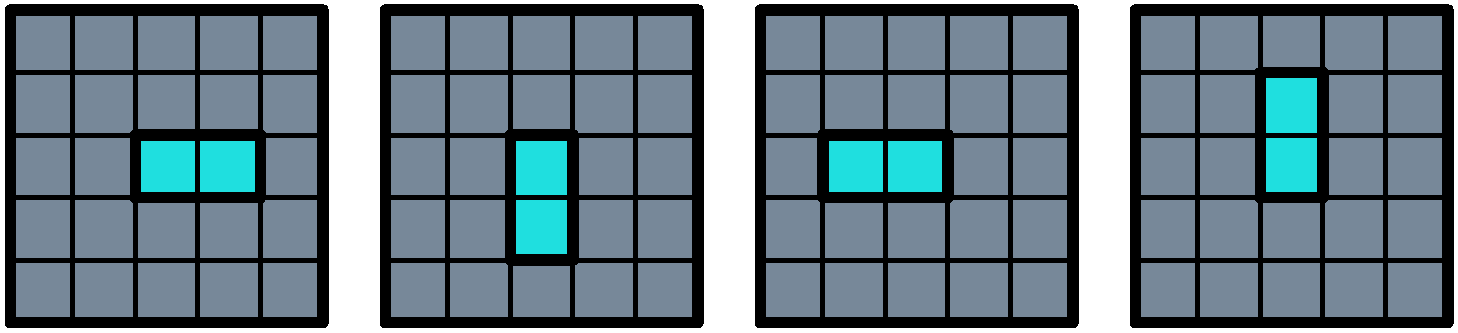
\includegraphics[width=0.6\textwidth]{./pictures/dominoes/mapping.pdf}
    \caption{The mapping of a piece placed at the center of the grid. From left to right, the orientations are \(0^\circ\), \(90^\circ\), \(180^\circ\), and \(270^\circ\), respectively.}
    \label{dom:mapping} 
\end{figure}

The moves for the dominoes contains the default drop $d$ and slides $s_r, s_l$ . For the fix move the \emph{partial lock out rule}\cite{WikiFandom} will be assumed, fixing only a piece if is entirely  inside the board. Regarding rotation moves, most modern Tetris implementations employ the Super Rotation System (SRS), the official Tetris Guideline standard for tetromino rotation behavior\cite{SRS}. In SRS, when a piece is rotated and overlaps with filled cells, the system attempts to reposition the piece by testing a predefined set of translations. 

\vspace{1em}

Following a similar approach, Dominoes Rotation System (DRS) is defined, described in Table~\ref{dom:rotation}. Intuitively, DRS tries to rotate a piece by moving it slightly depending on its orientation: \(r_+\) attempts to place the piece to the right or above, while \(r_-\) shifts it to the left or below, depending on its orientation. When a piece is rotated, DRS performs the following steps:
\begin{enumerate}
    \item First, DRS attempts the rotation using Test 1. 
    \item If the resulting piece overlaps with a filled cell, DRS proceeds to Test 2. 
    \item If Test 2 also fails, the piece cannot be rotated, and the move is deemed illegal.
\end{enumerate}


\begin{table}[ht]
\centering
\begin{tabular}{|c || c | c || c | c ||} 
 \hline
  & \multicolumn{2}{| c ||}{ $\VD$ } & \multicolumn{2}{| c ||}{$\HD$} \\
 \hline               
 & Test 1  & Test 2 & Test 1  & Test 2 \\ 
 \hline               
 $r_+$ & $\vcenter{\hbox{
\includegraphics[scale=0.3]{./pictures/dominoes/rotation/vert_clock_1.pdf}}}$ & $\vcenter{\hbox{
\includegraphics[scale=0.3]{./pictures/dominoes/rotation/vert_clock_2.pdf}}}$  & $\vcenter{\hbox{
\includegraphics[scale=0.3]{./pictures/dominoes/rotation/horit_clock_1.pdf}}}$  & $\vcenter{\hbox{
\includegraphics[scale=0.3]{./pictures/dominoes/rotation/horit_clock_2.pdf}}}$ \\ 
 \hline                             
 $r_-$ & $\vcenter{\hbox{
\includegraphics[scale=0.3]{./pictures/dominoes/rotation/vert_anti_1.pdf}}}$ & $\vcenter{\hbox{
\includegraphics[scale=0.3]{./pictures/dominoes/rotation/vert_anti_2.pdf}}}$  & $\vcenter{\hbox{
\includegraphics[scale=0.3]{./pictures/dominoes/rotation/horit_anti_1.pdf}}}$  & $\vcenter{\hbox{
\includegraphics[scale=0.3]{./pictures/dominoes/rotation/horit_anti_2.pdf}}}$ \\ 
 \hline
\end{tabular}
\caption{The DRS rotation table. The top rows indicate the initial orientation of the piece: vertical (\(\VD\)) or horizontal (\(\HD\)). The left columns specify the rotation direction (\(r_+\) for clockwise, \(r_-\) for counterclockwise), and the tests describe possible placements. In each image, the original piece is shown in white, while the resulting piece is displayed over it.}
\label{dom:rotation}
\end{table}


Figure~\ref{dom:drs} provides an example of the DRS rotation system in action.

\begin{figure}[ht]
  \centering
  \begin{subfigure}[b]{0.15\textwidth}
    \centering
    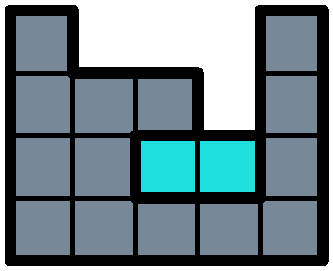
\includegraphics[width=0.9\textwidth]{pictures/dominoes/drs-1.pdf}
    \caption{}
  \end{subfigure}
  \begin{subfigure}[b]{0.15\textwidth}
    \centering
    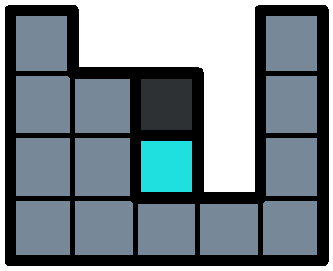
\includegraphics[width=0.9\textwidth]{pictures/dominoes/drs-2.pdf}
    \caption{}
  \end{subfigure}
  \begin{subfigure}[b]{0.15\textwidth}
    \centering
    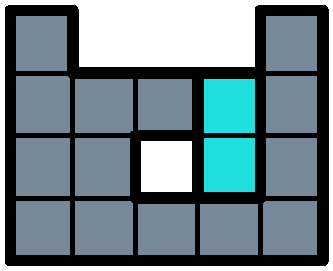
\includegraphics[width=0.9\textwidth]{pictures/dominoes/drs-3.pdf}
    \caption{}
  \end{subfigure}
  \caption{When rotating clockwise the domino in (a) DRS first ties to place it like (b), but this position isn't legal. Test 2 tries to place it in the right column which results a valid position.}
  \label{dom:drs}
\end{figure}

DRS allows pieces to move freely across the board, enabling not only standard movements but also upward motion in a staircase-like pattern, as shown in Figure~\ref{dom:staircase}. Most importantly, DRS makes it possible to place a domino in almost any position, despite the board configuration.

\begin{figure}
  \centering
  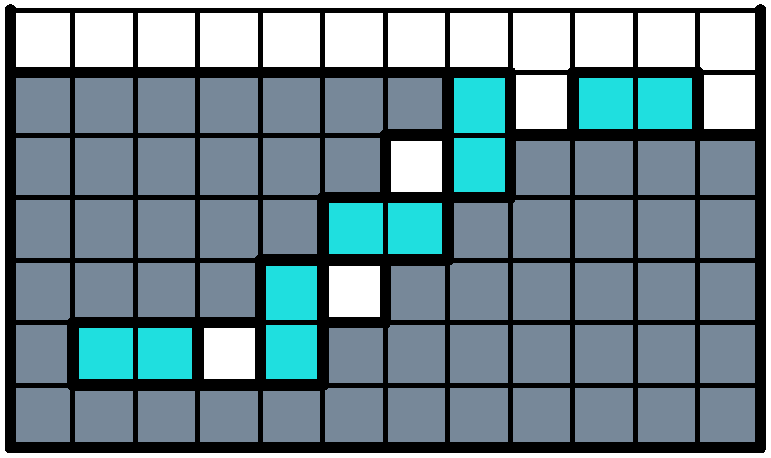
\includegraphics[width=0.3\textwidth]{pictures/dominoes/staricase.pdf}
  \caption{The overvevirew of a tragjectory starting at the left to the rightmost piece. The moves sequece is: $(3 \times s_r, 8 \times r_+, 2 \times s_r)$}
  \label{dom:staircase}
\end{figure}

\begin{definition}
  Let $B$ be a board in any configuration. A \emph{path} $p = (c_1,\dots , c_k) $ is a sequence of $k$ adjacent unfilled cells of $B$ where $c_1$ is a cell from the top row.
\end{definition}

\begin{lemma0} 
  Given a board $B$, exists a trajectory $\sigma$ for a domino that follows any path $p = (c_1,\dots , c_k) $ satisfying for any $ 1 < l < k $:
\begin{enumerate}
  \item if \(c_l = \cell\), \( c_{l+1} = \cell[i+1][j] \) and \( c_{l+2} = \cell[i+2][j] \), then either 
    \begin{enumerate}
      \item $\cell[i][j-1]$ is filled and cell $\cell[i+1][j-1]$ unfilled or \label{dom:path:up-left}
      \item $\cell[i][j+1]$ is filled and cell $\cell[i+1][j+1]$ unfilled \label{dom:path:up-right}
    \end{enumerate}
  \item $  c_l = \cell$, \( c_{l+1} = \cell[i+1][j] \) and \( c_{l+2} = \cell[i+1][j \pm 1] \), cell $\cell[i][j \pm 1]$ of $B$ is filled, respectively. \label{dom:path:turn} 
\end{enumerate}
\end{lemma0}
\begin{proof}
  Let \( p = (c_1, c_2, \dots, c_k) \) be such a path. Assuming that the domino is initially placed in cells \( c_1 \) and \( c_2 \) since the path starts at the top of the board. By proving that given a domino placed in \( c_l \) and \( c_{l+1} \) there exists a move, or a sequence of moves, that places the domino in \( c_{l+1} \) and \( c_{l+2} \) the entire trajectory can be constructed. 

  If $c_l = c_{l+2}$ no moves are needed. If \( c_l \), \( c_{l+1} \), and \( c_{l+2} \) are in the same row, a slide to the right $s_r$ or to the left $s_l$ places the domino in \( (c_{l+1}, c_{l+2}) \). When cells are in the same column and path goes downwards a drop $d$ does the job. If the path goes upwards, \ref{dom:path:up-left} or \ref{dom:path:up-right} must hold. Assuming \ref{dom:path:up-left} holds, the domino is moved from $c_l, c_{l+1}$ to $c_{l+1}, c_{l+2}$ with the following moves sequence:
  \[
    \vcenter{\hbox{
\includegraphics[width=0.05\textwidth]{pictures/dominoes/turns/up-1-0.pdf}}}
    \xrightarrow{r_-}
    \vcenter{\hbox{
\includegraphics[width=0.05\textwidth]{pictures/dominoes/turns/up-1-1.pdf}}}
    \xrightarrow{r_+}
    \vcenter{\hbox{
\includegraphics[width=0.05\textwidth]{pictures/dominoes/turns/up-1-2.pdf}}}
    \xrightarrow{s_r}
    \vcenter{\hbox{
\includegraphics[width=0.05\textwidth]{pictures/dominoes/turns/up-1-3.pdf}}}
    \hspace{3em}
    \vcenter{\hbox{
\includegraphics[width=0.05\textwidth]{pictures/dominoes/turns/up-2-0.pdf}}}
    \xrightarrow{r_-}
    \vcenter{\hbox{
\includegraphics[width=0.05\textwidth]{pictures/dominoes/turns/up-2-1.pdf}}}
    \xrightarrow{r_+}
    \vcenter{\hbox{
\includegraphics[width=0.05\textwidth]{pictures/dominoes/turns/up-2-2.pdf}}}
  \]

  The sequence of moves depends on the neighboring cells. When condition \ref{dom:path:up-right} is satisfied, the sequence $(r_+, r_+)$ places the domino in $c_{l+1}$ and $c_{l+2}$, regardless of the neighboring cells.

  Finally, the remaining cases are those where the path turns. There are four possible turns and each can be traversed in both directions, so there are eight scenarios. as shown in Figure~\ref{dom:turns}.

\begin{figure}[h]
  \centering
  \begin{subfigure}[b]{0.1\textwidth}
    \centering
    
\includegraphics[width=0.9\textwidth]{pictures/dominoes/turns/turn_1.pdf}
    \caption{}
    \label{dom:turn1}
  \end{subfigure}
  \begin{subfigure}[b]{0.1\textwidth}
    \centering
    
\includegraphics[width=0.9\textwidth]{pictures/dominoes/turns/turn_2.pdf}
    \caption{}
    \label{dom:turn2}
  \end{subfigure}
  \begin{subfigure}[b]{0.1\textwidth}
    \centering
    
\includegraphics[width=0.9\textwidth]{pictures/dominoes/turns/turn_3.pdf}
    \caption{}
    \label{dom:turn3}
  \end{subfigure}
  \begin{subfigure}[b]{0.1\textwidth}
    \centering
    
\includegraphics[width=0.9\textwidth]{pictures/dominoes/turns/turn_4.pdf}
    \caption{}
    \label{dom:turn4}
  \end{subfigure}
  \begin{subfigure}[b]{0.1\textwidth}
    \centering
    
\includegraphics[width=0.9\textwidth]{pictures/dominoes/turns/turn_5.pdf}
    \caption{}
    \label{dom:turn5}
  \end{subfigure}
  \begin{subfigure}[b]{0.1\textwidth}
    \centering
    
\includegraphics[width=0.9\textwidth]{pictures/dominoes/turns/turn_6.pdf}
    \caption{}
    \label{dom:turn6}
  \end{subfigure}
  \begin{subfigure}[b]{0.1\textwidth}
    \centering
    
\includegraphics[width=0.9\textwidth]{pictures/dominoes/turns/turn_7.pdf}
    \caption{}
    \label{dom:turn7}
  \end{subfigure}
  \begin{subfigure}[b]{0.1\textwidth}
    \centering
    
\includegraphics[width=0.9\textwidth]{pictures/dominoes/turns/turn_8.pdf}
    \caption{\label{dom:turn8}}
  \end{subfigure}
    \caption{The possible turns. The domino before the move is painted, and the destination cell is marked in white. The dark gray cell represents the corner of the turn, which alters the sequence of moves depending on whether it is filled or not.} 
    \label{dom:turns} 
\end{figure}
The trajectory required to perform the move involves either one or two steps, depending on the state of the corner cell. The remaining cells can be in any configuration. Table~\ref{dom:turns-table} shows the necessary moves for each scenario based on whether the corner cell is filled.

\begin{table}[ht]
\centering
\begin{tabular}{|c || c | c | c | c | c | c | c | c |} 
 \hline
  & \ref{dom:turn1} & \ref{dom:turn2} & \ref{dom:turn3} & \ref{dom:turn4} & \ref{dom:turn5} & \ref{dom:turn6} & \ref{dom:turn7} & \ref{dom:turn8} \\
 \hline               
  filled & $ r_-  $ & $      r_-    $ & $   r_+       $ & $   r_+       $ & $   r_+       $ & $     r_-     $ & $   r_-       $ & $   r_+      $  \\
 \hline               
unfilled & $ r_-  $ & $     -       $ & $   r_+, s_r  $ & $   r_+       $ & $    -        $ & $  r_-, s_r   $ & $   r_-       $ & $   r_+      $  \\
 \hline               

\end{tabular}
\caption{The moves needed to do each turn of Table~\ref{dom:turns}. When the corner cell is unfilled in \ref{dom:turn2} and in \ref{dom:turn5}, the condition \ref{dom:path:turn} is not satisfied. }
\label{dom:turns-table}
\end{table}

Each step can be calculated in constant time, so the path can be computed in $\mathcal{O}(k)$.

\end{proof}


\subsection{Constructible Boards}

In this work is assumed that boards initial configurations can be built within the game rules, starting from an empty board.  

\begin{definition}
  Given a Tetris game, a board $B$ configuration is \emph{constructible} configuration if exist a match $\Sigma = B_0, \sigma_1, B_1, \dots, B_k$ such that $B_0$ is empty and $B_k = B$. 
\end{definition}

The set of constructible configurations for a game variation is bigger as the game has more elements. For $1$\textsc{-Tris} all the boards look like a histogram, since each piece occupies one cell, and for the standard Tetris game almost all configuration are constructible \cite{HCTC}. Next follows a result for constructible boards in dominoes games that will be used in later proofs.

\begin{lemma0} \label{lem:floating}
  In any constructible board, for any filled cell $\cell$ at least on of the downward neighbors ($\cell[i-1][j-1]$, $\cell[i-1][j]$ and $\cell[i-1][j+1]$) must be filled.
\end{lemma0}  

\begin{proof}  
Let \(B\) be an \(n \times m\) board containing such a filled cell. Consider the sequence of boards \(B_0, B_1, \dots, B_k = B\), where \(B_0\) is an empty board and \(B_k = B\). Assume, without loss of generality, that \(B_k\) is the first board in the sequence containing a filled cell \(\cell_k\) (the cell \(\cell\) in \(B_k\)) such that the cells \(\cell[i-1][j-1]_k\), \(\cell[i-1][j]_k\), and \(\cell[i-1][j+1]_k\) are all unfilled.


The cell \(\cell_k\) cannot result from adding a domino that does not clear a row. Therefore, \(B_k\) must be obtained by adding a domino to \(B_{k-1}\) in such a way that it clears a row. Considering the row, the last placed domino, and the pieces used to achieve this, there are five possible ways of clearing a row:

\begin{figure}[ht]
  \centering
  \begin{subfigure}[b]{0.15\textwidth}
    \centering
    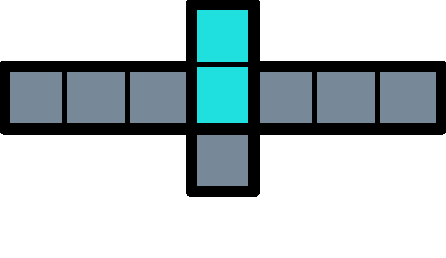
\includegraphics[width=0.9\textwidth]{./pictures/dominoes/proff-floating/clear-row-1.pdf}
    \caption{\label{dom:proff-floating:clear1}}
  \end{subfigure}
  \begin{subfigure}[b]{0.15\textwidth}
    \centering
    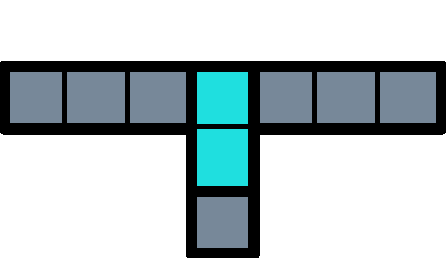
\includegraphics[width=0.9\textwidth]{./pictures/dominoes/proff-floating/clear-row-2.pdf}
    \caption{\label{dom:proff-floating:clear2}}
  \end{subfigure}
  \begin{subfigure}[b]{0.15\textwidth}
    \centering
    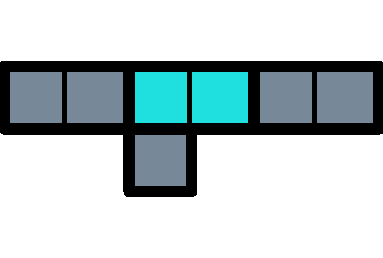
\includegraphics[width=0.9\textwidth]{./pictures/dominoes/proff-floating/clear-row-3.pdf}
    \caption{\label{dom:proff-floating:clear3}}
  \end{subfigure}
  \begin{subfigure}[b]{0.15\textwidth}
    \centering
    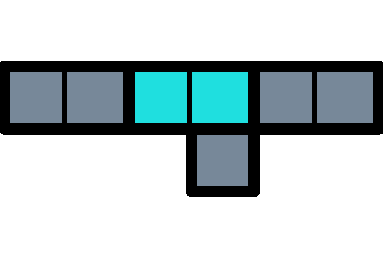
\includegraphics[width=0.9\textwidth]{./pictures/dominoes/proff-floating/clear-row-5.pdf}
    \caption{\label{dom:proff-floating:clear5}}
  \end{subfigure}
  \begin{subfigure}[b]{0.15\textwidth}
    \centering
    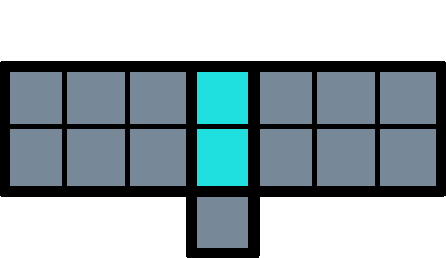
\includegraphics[width=0.9\textwidth]{./pictures/dominoes/proff-floating/clear-row-4.pdf}
    \caption{\label{dom:proff-floating:clear4}}
  \end{subfigure}
\end{figure}


  Let $r$ be the cleared row in \( B_{k-1} \), bottom cleared row in case \ref{dom:proff-floating:clear4}. Consider the board $B_{k-1}$ after placing the domino but before clearing the lines. Each cell $\cell[i'][j']$ from this board has the same downward neighbors as the cell $\cell[i'+1][j']_k$ ($i+2$ in case \ref{dom:proff-floating:clear4}) except for the cells just above the cleared row(s). Hence, cell \(\cell_k \) must be in row $r$: \( \cell_k = \cell[r]_k \).

  Any filled cell in $B_{k-1}$ has one of its downward neighbors filled, so if $\cell[r]_{k-1}$ is filled then $\cell[r]_k$ would have a downward neighbor filled, because cells below row $r$ aren't modified when clearing the row. Therefore, $\cell[r]_k$ can't be in a cell filled in $B_k$. This leads to few options:

\begin{figure}[ht]
  \centering
  \begin{subfigure}[b]{0.15\textwidth}
    \centering
    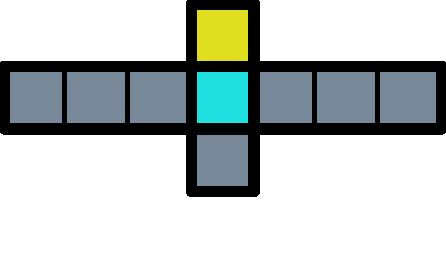
\includegraphics[width=0.9\textwidth]{./pictures/dominoes/proff-floating/scenario-1.pdf}
    \caption{}
    \label{floating:a}
  \end{subfigure}
  \begin{subfigure}[b]{0.15\textwidth}
    \centering
    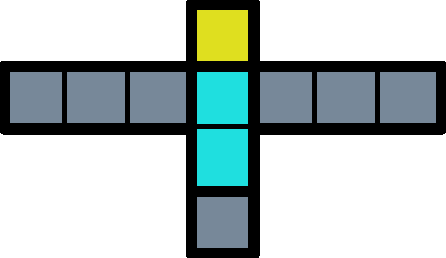
\includegraphics[width=0.9\textwidth]{./pictures/dominoes/proff-floating/scenario-2.pdf}
    \caption{}
    \label{floating:b}
  \end{subfigure}
  \begin{subfigure}[b]{0.15\textwidth}
    \centering
    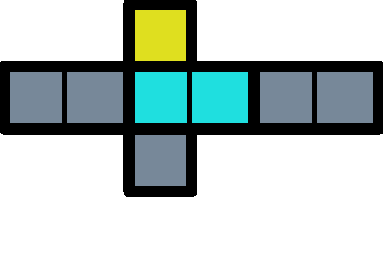
\includegraphics[width=0.9\textwidth]{./pictures/dominoes/proff-floating/scenario-3.pdf}
    \caption{}
    \label{floating:c}
  \end{subfigure}
  \begin{subfigure}[b]{0.15\textwidth}
    \centering
    \includegraphics[width=0.9\textwidth]{./pictures/dominoes/proff-floating/scenario-4.pdf}
    \caption{}
    \label{floating:d}
  \end{subfigure}
  \begin{subfigure}[b]{0.15\textwidth}
    \centering
    \includegraphics[width=0.9\textwidth]{./pictures/dominoes/proff-floating/scenario-5.pdf}
    \caption{}
    \label{floating:e}
  \end{subfigure}
  \linebreak
  \begin{subfigure}[b]{0.15\textwidth}
    \centering
    \includegraphics[width=0.9\textwidth]{./pictures/dominoes/proff-floating/scenario-6.pdf}
    \caption{}
    \label{floating:f}
  \end{subfigure}
  \begin{subfigure}[b]{0.15\textwidth}
    \centering
    \includegraphics[width=0.9\textwidth]{./pictures/dominoes/proff-floating/scenario-7.pdf}
    \caption{}
    \label{floating:g}
  \end{subfigure}
  \caption{Each picture represents the hole in row $r$ after placing the domino and before clearing the row. In yellow the cell candidate to fill $\cell[r]_k$. Blue cells correspond to the domino placed.}
\end{figure}

After clearing the row, none of the above cases succeed in creating the cell without downward neighbors, so such a cell can't appear in any board.
\end{proof}

Moreover, this lemma implies that in any constructible configuration, completely floating blocks--i.e., blocks whose lower corners do not touch any domino--cannot exist. 

\begin{corollary0}
  In any constructible configuration, each filled cell forms an uncrossable column down to the bottom of the board.
\end{corollary0}
\begin{proof}
  If a cell is filled, by Lemma~\ref{lem:floating}, one of its downward neighbors is filled. And his downward neighbor filled also has a downward neighbor filled, and so on until the bottom of the board. Due to the shape of the column, it cannot be crossed by any path.
\end{proof}

This characterization also provides insight into the possible arrangements of holes and paths within the board, making it useful for following proofs. The following corollary will help when filling the board. 

\begin{corollary0} \label{coro:fill-split}
  In any constructible configuration, for any path $p = (c_1, \dots, c_k)$ exists another $p' = (d_1, \dots, d_{k'})$ that starts and ends on same cells while not going upwards. Formally:
  \begin{enumerate}
    \item $c_1 = d_1$, $c_2 = d_2$, $c_{k-1} = d_{k'-1}$ and $c_k = d_{k'}$.
    \item for any $ 1 < l < k'-1$, if $d_l = \cell$ then $d_{l+1} \neq  \cell[i+1]$. \label{lemma:paths:cond2}
  \end{enumerate}

\end{corollary0}
\begin{proof}
  Let $p = (c_1, \dots, c_k)$ be such a path, and $c_l$ the last cell such that $c_l = \cell$ and $c_{l+1} = \cell[i+1]$. Let $c_m$ be the last cell of $p$ before $c_{l+1}$ at row $i+1$. Consider all cells in row $i+1$ between $c_l$ and $c_m$, as is show in the picture:

  $$ \includegraphics[width=0.4\textwidth]{./pictures/dominoes/equivalent-path.pdf} $$

  If any of these cells are filled, by Corollary~\ref{coro:fill-split}, no path could go under row $i+1$, hence between cells are empty. If $c_l = \cell[i+1][j']$, the new path that goes straight thought these cells is: 

  $$ p' = (c_1, \dots, c_m = \cell[i+1][j'], \cell[i+1][j'+1], \dots, \cell[i+1][j-1], \cell[i+1]= c_l, \dots c_k)$$

  when $ j' < j $, and analogously for $j < j'$. Repeating the argument for $p'$ until condition~\ref{lemma:paths:cond2} is satisfied the equivalent path is obtained.
\end{proof}


With the previous results a domino can be placed to any position of the board, but not fixed since the below cells can be unfilled. 

\subsection{Tetris Survival with Rotation}

The problem $\textsc{Tetris}\lbrack \VD \rbrack $ \survival\ can be formulated as follows: \emph{Given an arbitrarily sized board with an constructible initial configuration and a sequence of \( k \) dominoes, is there a way to play all the pieces while avoiding losing?} As pointed out\cite{TT}, if there exists a strategy to clear a single row, it is possible to survive indefinitely by employing the following piece-placement strategy:

\begin{enumerate}
    \item Rotate the piece to be vertical. 
    \item Place the piece in any column with the two top cells empty.
\end{enumerate}

To solve the problem it must be demonstrated that deciding whether any row can be cleared and, when not, compute the maximum number of pieces that can be fixed into the board before losing can both be computed in polynomial time. The problem will be addressed in these three parts separately, and then the results will be combined.  

\vspace{1em}
To clear a row, dominoes must be fixed into specific board positions. The following result shows that determining whether a domino can be placed in a given position can be checked in polynomial time.

\begin{lemma0}
 Let $B$ be an $n\times m $ board, and let $p$ be a path in $B$. Checking if exists a match $\Sigma = B,\sigma_1, B_1, \sigma_2, \dots, \sigma_k, B_k$ such that $\sigma_k$ fixes a domino in any position of the path $p$ can be computed in $\mathcal{O}(n)$.  
\end{lemma0}
\begin{proof} 
  Let $(c_1, c_2)$ be the desired position in the path. Without loss of generality assume that the path $p$ ends with $(c_1, c_2)$.  Also assume that $p$ doesn't go upwards, by considering the equivalent path provided by Lemma~\ref{coro:fill-split}.

  Since $(c_1, c_2)$ are in the end of a path, by Lemma~\ref{dom:path:turn} exists a trajectory $\sigma$ that places a domino in $(c_1, c_2)$. The piece now needs to be fixed. If the cell below $c_1$ or the cell below $c_2$ is filled the domino can be fixed directly. Otherwise, when the domino can't be fixed one of the below pieces has to be filled. When the domino is horizontally orientated it can be fixed by repeteadly placing the domino in $(c_1, c_2)$ with $\sigma$ and hard dropping it eventually a domino will be fixed in $(c_1, c_2)$.

  \[
    \vcenter{\hbox{\includegraphics[width=0.04\textwidth]{pictures/dominoes/proff-fix/horti-1.pdf}}}
    \xrightarrow{d_h}
    \vcenter{\hbox{\includegraphics[width=0.04\textwidth]{pictures/dominoes/proff-fix/horti-2.pdf}}}
    \xrightarrow{d_h}
    \vcenter{\hbox{\includegraphics[width=0.04\textwidth]{pictures/dominoes/proff-fix/horti-3.pdf}}}
    \xrightarrow{d_h}
    \vcenter{\hbox{\includegraphics[width=0.04\textwidth]{pictures/dominoes/proff-fix/horti-4.pdf}}}
    \xrightarrow{d_h}
    \vcenter{\hbox{\includegraphics[width=0.04\textwidth]{pictures/dominoes/proff-fix/horti-5.pdf}}}
  \]

  If $(c_1, c_2)$ are in row $i$ and the first filled cell bellow $c_1$ and $c_2$ is in row $i'$, the match is:

  $$ \Sigma = B, (\sigma, d_h), B_1, \dots,B_{i-i'-1},  (\sigma, d_h), B_{i-i'}  $$

  Where the hard drop can be decomposed into the sequence of drops and fix if isn't available in the move set. In this scenario the domino can be always fixed in $(c_1, c_2)$.

  Finally, the case where $(c_1, c_2)$ are vertically orientated. If $c_1 = \cell$ and $c_2 = \cell[i+1]$, the cell $\cell[i-1]$ must be also filled to fix the domino in $(c_1, c_2)$. This can be achived by placing another domino into one of the following:
\[
  \begin{array}{c@{\hspace{-0.5em}}cc@{\hspace{-0.5em}}cc@{\hspace{-0.5em}}c}
    \begin{minipage}{0.08\textwidth}
      \includegraphics[width=\textwidth]{pictures/dominoes/proff-fix/vert-1.pdf}
    \end{minipage} &
    \begin{minipage}{0.2\textwidth}
      \center
      \(\cell[i-1][j-1], \cell[i-1][j]\)
    \end{minipage} &
    \begin{minipage}{0.08\textwidth}
      \includegraphics[width=\textwidth]{pictures/dominoes/proff-fix/vert-3.pdf}
    \end{minipage} &
    \begin{minipage}{0.15\textwidth}
      \center
      \(\cell[i-1][j], \cell[i-2][j]\)
    \end{minipage} &
    \begin{minipage}{0.08\textwidth}
      \includegraphics[width=\textwidth]{pictures/dominoes/proff-fix/vert-2.pdf}
    \end{minipage} &
    \begin{minipage}{0.2\textwidth}
      \center
      \(\cell[i-1][j], \cell[i-1][j+1]\)
    \end{minipage}
  \end{array}
\]
 
  If any of the before dominoes can be fixed into its position, then domino can be fixed into $c_1,c_2$. The overall procedure is the following: 


  \begin{algorithm}
  \begin{algorithmic}
    \Procedure{CanBeFixed}{$B, c_1 = \cell, c_2 = \cell[i'][j']$}\Comment{$c_1, c_2$ adjacent cells in $B$}
      \If{$\cell[i][j]$ or $\cell[i'][j']$ filled} 
        \State \Return False  \Comment{$c_1$ or $c_2$ are filled}
      \ElsIf{$\cell[i-1][j]$ or $\cell[i'-1][j']$ unfilled}
        \State \Return True \Comment{the domino can be directly fixed}
      \ElsIf{$ i = i'$}
        \State \Return True \Comment{an horizontal domino can always be placed below}
      \EndIf
      \State $c_2 = \cell[i+1][j]$ \Comment{$c_1$ and $c_2$ are vertically aligned}
      \State \Return \Call{CanBeFixed}{$B$, $\cell[i-1]$, $\cell[i-2]$} 
    \EndProcedure
  \end{algorithmic}
  \end{algorithm}


  In worst case scenario the algorithm does $n / 2$ calls of constant cost, since in each call the row is decreased by two. Hence, the total cost is $\mathcal{O}(n)$.

\end{proof}

Note that the proof doesn't if any row is cleared when filling the board, this is because the goal is to fully fill a row. If at some point a row is cleared then the goal would be acomplished. Now we are ready to solve the main question of $\textsc{Tetris}\lbrack \VD \rbrack $ \survival. 

\begin{lemma0} \label{dom:clear-top}
For any $n \times m$ board, deciding whether the top row can be cleared is in \pp.
\end{lemma0}
\begin{proof}
\end{proof}

\begin{lemma0} \label{dom:clear-row}
For any $n \times m$ board, deciding if any row, except the first one, can be cleared is in \pp.
\end{lemma0}

\begin{proof}
  % Let $r < m$ be the row to be checked. To fill completely the row all the holes need to be fully filled. Let $h = \{ \cell[r][j_1], \dots, \cell[r][j_2]\}$ a hole in row $r$ from column $j1$ to column $j_2$.  
\end{proof}


\begin{lemma0} \label{dom:max-fill}
  Let $B$ be a board such that no row can be cleared. The maximum number of dominoes that can be fixed into the board before loosing can be computed in $\mathcal{O}(??)$.
\end{lemma0}

\begin{proof}
\end{proof}

\begin{theorem}
  \textsc{2-tris} \survival is in \pp.
\end{theorem}

\begin{proof}
\end{proof}

\subsection{Clearing without rotation}

The proof is a reduction from \textsc{3-Partition} and takes a similar approach as the first Tetris proof\cite{TIH} and other later ones\cite{TT, TWFP, TCB, CTV}. The \textsc{3-Partition} problem is defined as follows:

\textbf{Input:} Given a multiset of positive integers $A = \{ a_1, a_2, \dots, a_{3m} \}$ such that:

$$ \frac{t}{4} < a < \frac{t}{2}\;\; \forall a \in A \text{, where } t = \frac{1}{m} \sum_{i=1}^{3m} a_i $$ 

\textbf{Output:} Decide whether the set can be partitioned into $m$ subsets $D_1, \dots D_m$, each of size $3$ and summing $t$. 

$$ | D_i | = 3 \text{ and } \sum_{a \in D_i} a = t\text{   } 1 \leq i \leq m$$

\begin{theorem} 
  \textsc{2-{Tris-NoRotation}} \clearing\ is \npc.
\end{theorem}

\begin{proof}
  \textbf{TO FINISH: pictures need impovement}

  Let \( A = \{ a_1, a_2, \dots, a_{3m} \} \) be an instance of the \textsc{3-Partition} problem with \( t \) as defined. Construct the corresponding instance of \textsc{2-Tris-NoRotation} as follows:

  The board \( B \) is made up attaching horizontally \( m \) \emph{buckets}. A bucket consists of five adjacent columns, each of height \( 3m + 2t \). The first and fifth column of a bucket are filled, the third one is empty and second and fourth columns have filled the following cells:
  $$ 
    \{ \cell[2][j] \mid j \leq 2t \text{ or } j \text{ odd}\} \cup
    \{ \cell[4][j] \mid j \leq 2t \text{ or } j \text{ even}\}
    $$
  the top $3m$ rows will be refered as blocking rows and the $2t$ bottom rows as filling rows. The number of empty cells is $3m + 2t + 3m = 2(3m + t)$, so the number of filled cells in the whole board is $2m(3m + t)$. In the reduction, each bucket corresponds to one of the answer sets $D_i$, which will be filled while playing the game. The board looks like: 
  \[
    \underbrace{
    \begin{array}{c@{\hspace{0px}}c@{\hspace{0px}}c@{\hspace{0px}}c}
      \underbrace{\vcenter{\hbox{\includegraphics[width=0.1\textwidth]{./pictures/dominoes/proff-nph/bucket.pdf}}}}_{\text{bucket}}
      &
      \underbrace{\vcenter{\hbox{\includegraphics[width=0.1\textwidth]{./pictures/dominoes/proff-nph/bucket.pdf}}}}_{\text{bucket}}
      &
      \cdots 
      &
      \underbrace{\vcenter{\hbox{\includegraphics[width=0.1\textwidth]{./pictures/dominoes/proff-nph/bucket.pdf}}}}_{\text{bucket}}  
    \end{array}
  }_{m \text{ buckets}}
  \]

 The piece sequence consists on a sequence of vertical ($\VD$) or horizontal ($\HD$) dominoes. Each $a_i$ is encoded in sequence of dominoes and the sequence is obtained by attaching each $a_i$ encoded. Each $a_i$ is encoded as:
 \[
  S(a_i) \mapsto S_i = 
  ( \underbrace{\HD, \dots, \HD}_{m-1}, \underbrace{\VD, \dots, \VD}_{a_i}, \HD )
 \]
 The first $m-1$ dominoes will be referred as the priming sequence, the next $a_i$ dominoes as filling sequence and finally the clearing piece. So the piece sequence for the game is $ S = S_1 S_2 \dots S_{3m}$. The total number of cells of the dominoes sequence is
 \[
  2 \sum_{a_i \in A} (m-1) + a_i + 1 = 6m^2 + 2\sum_{a_i \in A} a_i = 6m^2 + 2mt = 2m(3m+t)
 \]

 which corresponds to the number of empty cells of the board, hence in order to clear the hole board each domino must be placed in the board holes. Moreover, dominos of the filling sequence can only be placed at the bottom of the filling rows and the priming sequence in the top row of the blocking rows.

 The first $m-1$ pieces of the sequence are $\HD$ that must be placed in the top row. Not placing any of the dominos in such position forces to place the piece in one row above, making the clearing impossible. After placing the $m-1$ all the buckets except one have the top row filled. Let $j$ be this bucket.

 \begin{center}
 \includegraphics[width=0.7\textwidth]{./pictures/dominoes/proff-nph/top-row-filled.pdf}
 \end{center}

 Next follows $a_1$ vertical dominoes that can only be placed in the middle column of the $j$ bucket, because any other position forces to fill a cell in a row above. Finally, the clearing piece must be placed in the bucket $j$, by the same argument, clearing the top row. After placing the first $m + a_1$ pieces of the sequence, the ones corresponding to $S_1$, $a_i$ dominoes have been added to the bottom of a bucket $j$ and the first row cleared.

 $$ picture $$

 Next follows $S_2$ and so on. If at some point the filling sequence of some $S_i$ overfills the filling rows, a $\VD$ is placed in a blocking row impeding the afected blocking rows to be cleared by $\HD$, so clearing is impossible.

 \begin{center}
 \includegraphics[width=0.7\textwidth]{./pictures/dominoes/proff-nph/overfill.pdf}
 \end{center}



\end{proof}

\subsection{Towards Clearing}
\subsection{Tetris with Vertical Dominoes}

Using the notation introduced earlier, the problem is as $\textsc{Tetris-NoRotation}\lbrack \VD \rbrack$, considering both \clearing\ and \survival. The input consists of a sequence of vertical dominoes and an arbitrarily sized $n \times m$ board in a constructible configuration. The initial state function in this variation differs from the default orientation, as the pieces must be from the beginning in a vertical orientation.

\subsubsection{Constructible board configurations}

First we will to characterize the constructible boards with $\VD$ pieces without rotation by exploring the configuration starting from an empty board. 

Vertical dominoes consist of two vertical adjacent cells, so for an empty board any trajectory fixes the piece in the bottom row, filling $\cell[1][i]$ and $\cell[2][i]$ cells for any $1 \leq i \leq m$. The next domino can either go to an empty column or to the one before. Placing the first $m$ dominoes in unfilled columns clears the two lowest rows, and consequently the board. When a domino is placed in a non-empty column $i$, the $\cell[3][i]$ and $\cell[4][i]$ are filled, and so on, util a $\VD$ is placed in the last unfilled column. When this happens the two lowest rows are cleared and the process continues. 

So we can represent a reachable configuration of a given $n \times m$ board $B$ with a sequence of $m$ integers $(a_1, \dots, a_m)$, where

$$0 \leq a_i \leq \lceil \frac{n}{2} \rceil, \;\;\;   \forall i = 1,\dots, m$$

and $\exists i$ such that $a_i = 0$ (an empty column), with the following mapping: 

$$
\cell = \begin{cases}
   \text{filled}  & \text{if } i \leq  2a_j  \\
   \text{empty}   & \text{if } i >  2a_j
\end{cases}
$$

Each $a_i$ counts the number of vertical pieces placed in the column $i$. For example, in a $10 \times 6 $  board, the sequence $(1,2,0,4,2,3)$ defines the configuration in 
\ref{dom:vconf}.

\begin{figure}[ht]
  \centering
  \begin{subfigure}[b]{0.2\textwidth}
    \centering
    \includegraphics[width=0.9\textwidth]{pictures/dominoes/vertical_configuration.pdf}
    \caption{}
  \end{subfigure}
  \begin{subfigure}[b]{0.2\textwidth}
    \centering
    \includegraphics[width=0.9\textwidth]{pictures/dominoes/vertical_configuration_filled.pdf}
    \caption{}
  \end{subfigure}
    \caption{The $10 \times 6 $ board configuration represented by the sequence $(1,2,0,4,2,3)$, in yellow the 13 dominoes needed to clear the board.}
  \label{dom:vconf}
\end{figure}

\subsubsection{Cleaing}

In this decisional problem the input is a sequence of $k$ vertical dominoes and an $n \times m$ board with an initial configuration, that can be represented by the sequence $(a_1, \dots, a_m)$ as before. The question is: \emph{Is ther a way to clean the board after placing the $k$ pieces?}

\begin{theorem} 
$\textsc{Tetris-NoRotation}\lbrack \VD \rbrack $ \clearing\ is in \pp.
\label{dom:no-rot-vd}
\end{theorem}
\begin{proof}
    Let $B = (a_1, \dots, a_m) $ be the board representation and $k$ the length of the sequence of vertical dominoes. For every constructible board there is an empty column, so the strategy consists on placing each piece in an arbitrary empty column. 

    All the empty cells under the lowest empty row need to be filled to clean the board. Let $a_{\max}$ be the max in the board representation. Since we fill cells with dominoes, the number of dominoes $k_{\min}$ needed to clean the board is:
    $$ k_{\min} = \sum_{i = 1}^m \left( a_{\max} - a_i \right) $$

    If $k < k_{\min}$ we can't clear the board. If $k =  k_{\min}$ we can clear the board. And when $k > k_{\min}$, we can clean the board if after placing $k_{\min}$ dominoes the number of remaining pieces is a multiple of the board width, $k - k_{\min} \equiv 0 \mod m$. Since all the computations can be done in polyatomic time in respect of the input, the problem is in \pp.
\end{proof}

For boards with an even number of rows all pieces always fit inside the board. For an odd number of rows, dominoes could be placed in the top row with half of the domino inside the board and half outside. If we allow this, by changing the \emph{fix} function, the result would be the same since the same strategy works. The Figure~\ref{dom:vconf} shows, in yellow color, how the number of pieces needed to clean the board.

\subsubsection{Survival}

With the same input, the objective is to do not lose. The last proof provides a strategy to survive indefinitely. So for any number of pieces $k$ there is a way to avoid losing. Hence:
\begin{theorem} 
$\textsc{Tetris-NoRotation}\lbrack \VD \rbrack $ \survival\ is in \pp.
\end{theorem}


\subsection{Tetris with horizontal dominoes}

As before, the problem is $\textsc{Tetris-NoRotation}\lbrack \HD \rbrack$, considering both \clearing\ and \survival. Placing a horizontal domino fills two adjacent cells in one row or clears the row, meaning each domino placed can be tracked until the row is cleared. Thus, for any initial constructible configuration, the filled cells can be uniquely grouped into dominoes, allowing us to refer to dominoes instead of individual filled cells.

Additionally, in any constructible board, each row must contain an even number of filled cells. Consequently, when the board width is odd, no row can be cleared. In such cases, the board can only be cleared if it starts as an empty board with an empty sequence of pieces. From this point onward, we will assume that the board has an even number of columns. 

Let $B$ be a board with $m$ columns. We divide the board into $m/2$ \emph{buckets}, where each bucket consists of a pair of consecutive columns. Then:

\begin{lemma0}   
    Not placing a domino inside a bucket makes the row unclearable.
\end{lemma0}
\begin{proof}
    Let $r$ be a row containing some dominoes. When a domino is placed in a bucket it divides the row into two parts: the cells on the left side of the domino and the ones on the right. Both parts of even length, and containing an even number of filled cells.

    In the other case the two parts have an odd length but containing an eaven number of filled cells, making them impossible to clean
    since there's no way to add an odd number of cells by placing dominoes.
\end{proof}

For example, in the Figure~\ref{dom:buckets}, the second piece occupies the second and the third bucket, making the row un-clearable. 

\begin{figure}[h]
    \centering
    \includegraphics[width=0.2\textwidth]{./pictures/dominoes/buckets.pdf}
    \caption{A board with one partially filled row.}
    \label{dom:buckets} 
\end{figure}


We now can prove both clearing and survival problems.

\begin{theorem}
    $\textsc{Tetris-NoRotation}\lbrack \HD \rbrack $ \clearing\ is in \pp.
\end{theorem}
\begin{proof}


    The input is an $n \times m$ input board $B$, filled with a construable configuration, and sequence of $k$ dominoes $\HD$. If $m$ is odd then the board can't be cleared if $k > 0$ or the initial board isn't empty. 

    When $m$ is even we first need to check if the board is clearable. If there's only one row, checking that the row has been built by placing each piece inside a bucket determines if the row is clearable. When the board has more than one row the same happens. 

    We first group in pieces the filled cells of each row from the initial board. This can always be done because there's no way to clean \emph{"half"} piece. Then we check if each piece is placed inside a bucket. If some piece isn't placed inside a bucket the board can't be cleared. We can compute this in $\mathcal{O}(n\cdot m)$.

    Now the board can be represented with a sequence $(a_1, \dots, a_{m/2})$ of $m/2$ numbers each representing the number of dominoes placed in each bucket.

    $$
    \cell = \begin{cases}
        \text{filled}  & \text{if } i \leq  a_{2j}  \\
        \text{empty}   & \text{if } i >  a_{2j}
    \end{cases}
    $$

    With some $a_i = 0$. Let $a_{\max} = \max \{a_1, \dots a_{m/2}$ \} be the maximum of the sequence. The minimum number of pieces needed to clear the board is:

    $$ k_{\min} = \sum_{i = 1}^{m/2} (a_{\max} - a_i )$$

    If $k < k_{\min}$ the board can't be cleared. If $k = k_{\min}$ the board can be cleared. When $k > k_{\min}$ the board can be cleared if $ k - k_{\min} \equiv 0 \mod m / 2$, sine the remaining pieces have to leave the board empty by filling rows.
\end{proof}

\begin{figure}[ht]
  \centering
  \begin{subfigure}[b]{0.2\textwidth}
    \centering
    \includegraphics[width=0.9\textwidth]{pictures/dominoes/horitzonatl_configuration_1.pdf}
    \caption{}
  \end{subfigure}
  \begin{subfigure}[b]{0.2\textwidth}
    \centering
    \includegraphics[width=0.9\textwidth]{pictures/dominoes/horitzonatl_configuration_2.pdf}
    \caption{}
  \end{subfigure}
  \begin{subfigure}[b]{0.2\textwidth}
    \centering
    \includegraphics[width=0.9\textwidth]{pictures/dominoes/horitzonatl_configuration_3.pdf}
    \caption{}
  \end{subfigure}
  \caption{Some board configurations. In (a) the board can't be cleared because the topmost domino is placed between the first and the second bucket. In (b) the board is represented by the sequence $(2,4,1,0,3)$, it can be cleared. The minimum number of pieces to clean the board is 10, this pieces appear in yellow in (c).}
  \label{dom:horitzonatl_configuration}
\end{figure}

Figure~\ref{dom:horitzonatl_configuration} shows some examples of the above prof. Next follows the \survival. In this scenario the goal is to find a strategy to survive indefinitely, to survive indefinitely.  

\begin{theorem}
    $ \textsc{Tetris-NoRotation}\lbrack \HD \rbrack $ \survival\ is in \pp.
\end{theorem}
\begin{proof}
    
If a given board \( B \) contains a clearable row, we can survive indefinitely by first clearing this row and then continuing to place pieces to refill the topmost row. If no such row exists---for instance, on a board with odd width---there exists a maximum number \( k_{\max} \) of dominoes that can be placed before a loss becomes inevitable. Thus, if the input length \( k \) is less than or equal to \( k_{\max} \), survival is possible; otherwise, it is not. The following procedure checks if any row can be cleared and, if not, computes \( k_{\max} \).

Horizontal dominoes fit naturally in a row, so maximizing the number of dominoes placed on the board \( B \) requires maximizing their placement in each row. To avoid blocking further placements, the board is filled from the bottom to the top. Within a row, a \emph{hole} is defined as a set of contiguous empty cells bounded by filled cells or the board's edges. 

% More formally, for row \( r \), a \emph{hole} is a segment:
%
% \[h^r_{j_1,j_2} = \{\cell[r][j_1], \cell[r][j_1+1], \dots, \cell[r][j_2]\}\]
%
% where all cells in \( h \) are empty, and the boundary cells \( \cell[r][j_1-1] \) and \( \cell[r][j_2+1] \) are either filled or lie outside the board.

To maximize the number of dominoes in the board, each row's holes must be filled as completely as possible. This reduces the problem of filling the entire board to the simpler task of optimally filling individual row holes. By systematically filling holes from the bottom-most row upwards, we ensure the greatest number of dominoes are placed without causing unresolvable blocking and ensure that each hole is above a maximally filled row. 

Let \( h = \{\cell[r][j_1], \cell[r][j_1+1], \dots, \cell[r][j_2]\} \) represent a hole in row \( r \) spanning columns \( j_1 \) to \( j_2 \). All cells in \( h \) are empty, and the boundary cells \( \cell[r][j_1-1] \) and \( \cell[r][j_2+1] \) are either filled or lie outside the board. To place a domino inside the hole, there must exist a trajectory from the top of the board to \( h \), making only reachable holes relevant for consideration.

Using Lemma~\ref{lem:floating} a hole must take one of the following shapes:

\begin{figure}[ht]
  \centering
  \begin{subfigure}[b]{0.24\textwidth}
    \centering
    \includegraphics[width=0.9\textwidth]{pictures/dominoes/simple-hole-1.pdf}
    \caption{}
    \label{dom:hole-a}
  \end{subfigure}
  \begin{subfigure}[b]{0.24\textwidth}
    \centering
    \includegraphics[width=0.9\textwidth]{pictures/dominoes/simple-hole-2.pdf}
    \caption{}
    \label{dom:hole-b}
  \end{subfigure}
  \begin{subfigure}[b]{0.24\textwidth}
    \centering
    \includegraphics[width=0.9\textwidth]{pictures/dominoes/simple-hole-3.pdf}
    \caption{}
    \label{dom:hole-c}
  \end{subfigure}
  \begin{subfigure}[b]{0.24\textwidth}
    \centering
    \includegraphics[width=0.9\textwidth]{pictures/dominoes/simple-hole-4.pdf}
    \caption{}
    \label{dom:hole-d}
  \end{subfigure}
  \label{dom:holes}
\end{figure}

Let \( l = j_2 - j_1 + 1 \) denote the length of the hole \( h \). The maximum number of dominoes that can be placed in holes of type \ref{dom:hole-a} and \ref{dom:hole-c} is \( \lfloor l / 2 \rfloor \) for $l > 2 $, completely filling the hole if \( l \) is even. For a hole of type \ref{dom:hole-b}, the same rule applies for \( l > 4 \). For $l = 4$ only one domino can be placed, as shown in Figure~\ref{dom:hole-4}.

\begin{figure}[h]
    \centering
    \includegraphics[width=0.18\textwidth]{./pictures/dominoes/hole-4.pdf}
    \caption{A type-\ref{dom:hole-b} hole of length 4.}
    \label{dom:hole-4} 
\end{figure}

Finally, the algorithm to decide the problem would look like:
\begin{algorithmic}[1]
    \Function{Tetris-NoRotation[$\HD$]}{$B,k$} \Comment{a board $B$ and $k$ dominos}
    \State $k_{\max}\gets 0$ \Comment{tracks if each hole of a row is fully filled}

    \For{row $r = 1, \dots, n$}
    \State $\text{full} \gets \text{True}$
      \For{hole $h$ in $r$}
        \State $k = \text{MaxDominoes}(h)$ \Comment{the $k$ dominoes that can be maximally placed in $h$}
        \If{$2 \cdot k_r \neq \text{length}(h)$}
          \State $\text{full} \gets \text{False}$
        \EndIf
        \State $k_{\max} = k_{\max} + k$
      \EndFor

      \If{ $\text{full}$}
        \State \textbf{return} $\text{True}$ \Comment{surviving indefinitely}
    \EndIf
\EndFor

\State \textbf{return} $k \leq k_{\max}$
\EndFunction
\end{algorithmic}

The cost of the algorithm is $\mathcal{O}(n \cdot m)$, since looping throught the holes has cost $\mathcal{O}(m)$ and filling the hole maximally has constant cost when the hole shape is known.

\end{proof}






\bibliographystyle{plain}
\bibliography{references} 

\end{document}
